\chapter{ASSIMILAÇÃO DE DADOS HÍBRIDA ENSEMBLE-VARIACIONAL GLOBAL}
\label{cap:incorpora_covars}

Neste capítulo é apresentada a metodologia para a incorporação das covariâncias do filtro de Kalman por conjunto (Seções \ref{sec:enkf} e \ref{sec:ensrf}) na estrutura variacional do sistema GSI (Seção \ref{sec:3dvar}). O código computacional dos sistemas EnKF e EnSRF já havia sido previamente programado e estava sendo testado pelo GMAO em suas aplicações de pesquisa no sistema híbrido proposto por eles. Para o caso do sistema híbrido 3DVar do CPTEC em uso com o modelo de circulação geral do centro, não foram necessárias modificações no código computacional, com excessão do tratamento do ozônio sendo este ajustado para ser univariado (i.e., não é considerada a sua covariância com as demais variáveis da matriz de covariâncias). Isso foi necessário devido aos problemas iniciais que foram encontrados com a representação do ozônio na matriz de covariâncias calculada para o MCGAv4.

Na seção a seguir é apresentada a metodologia de incorporação das covariâncias do filtro de Kalman por conjunto na estrutura variacional. Esta metodologia segue as ideias introduzidas por \citeonline{lorenc/2003} e aplicadas por \citeonline{wangetal/2008a,wangetal/2008b,wang/2010} no sistema GSI. A notação das equações foi alterada para ficar em conformidade com os demais desenvolvimentos apresentados no trabalho. Além da apresentação da metodologia para a incorporação das covariâncias, são apresentadas também as configurações utilizadas no sistema para que fosse possível realizar o ciclo de análises e previsões de forma satisfatória, o que inclui a determinação de parâmetros fundamentais para a assimilação de dados como a configuração das iterações da minimização da função custo, o controle da umidade não física, porcentagem de contribuição das covariâncias do conjunto entre outros. É apresentado também um diagrama esquemático ilustrando o ciclo de assimilação de dados do sistema híbrido. Neste diagrama são apresentadas também as principais equações envolvidas nas diferentes etapas do processo. Ao final do capítulo, é apresentado como é feita a análise do campo de vento horizontal no GSI, uma vez que diferentes quantidades para representar o vento estão envolvidas no processo de assimilação de dados e previsão.

\section{Incorporação das Covariâncias do filtro de Kalman por conjunto na Estrutura Variacional do GSI}

A técnica utilizada para incorporar as covariâncias dos erros de previsão provenientes do filtro de Kalman por conjunto (EnKF/EnSRF) na estrutura variacional tridimensional (3DVar) do GSI, é aquela apresentada por \citeonline{lorenc/2003} denominada ``Variável de Controle Alpha'' e também em \citeonline{wangetal/2008a,wangetal/2008b,wang/2010} denominada ``Variável de Controle Estendida''. A técnica de incorporação ou inclusão das covariâncias dos erros de previsão na estrutura variacional consiste na definição de um novo incremento de análise ($\delta{\mathbf{x}}'$) e de uma matriz de correlações ($\mathbf{C}$), cujos elementos são multiplicados pelos elementos da matriz de covariâncias dos erros de previsão proveniente do filtro de Kalman por conjunto ($\mathbf{P}^{b}$). Esta abordagem é semelhante aquela empregada nos trabalhos de \citeonline{claytonetal/2012} e \citeonline{wangelei/2013}. 

No sistema híbrido, o novo incremento de análise denotado por $\delta{\mathbf{x}}'$ é a soma de dois termos, definida como:

\begin{equation}
\label{eq:29}
\delta{\mathbf{x}'} = \delta{\mathbf{x}} + \sum_{k=1}^{K}{(\mathbf{x}_{k}^{e} \circ \mathbf{a}_{k})}
\end{equation}

onde:

\begin{itemize}
    \item $\delta{\mathbf{x}'}$: é o novo incremento de análise híbrido (dimensão: $n$ x $1$);
    \item $\delta{\mathbf{x}}$: é o incremento de análise original (i.e., $\mathbf{x}^{a}-\mathbf{x}^{b}$; $n$ x $1$);
    \item $\mathbf{a}_{k}$: é a extensão da variável de controle a ser analisada para cada membro do conjunto de $K$ previsões ($n$ x $k$);
    \item $\mathbf{x}_{k}^{e}$: é a $k$-ésima previsão do conjunto ($n$ x $1$).
\end{itemize}

Na Eq. \ref{eq:29}, o primeiro termo do lado direito da equação ($\delta{\mathbf{x}}$), é o incremento de análise associado com a covariância estática do erro de previsão ($\mathbf{B}$). O segundo termo ($\sum_{k=1}^{K}{\mathbf{x}_{k}^{e} \circ \mathbf{a}_{k}}$), é o incremento associado as covariâncias ($\mathbf{P}^{b}$) provenientes do filtro de Kalman por conjunto. Os vetores $\mathbf{a}_{k}$ (com $k=1,...,K$), denotam as extensões das variáveis de controle para cada membro (os quais serão explicados com mais detalhes adiante). O símbolo $\circ$ representa o produto Schur (i.e., elemento a elemento) entre os elementos dos vetores $\mathbf{a}_{k}$ e $\mathbf{x}_{k}^{e}$. Em outras palavras, o segundo termo na Eq. \ref{eq:29}, representa a combinação linear local das perturbações do conjunto com o incremento de análise original ($\delta{\mathbf{x}}$). O coeficiente $\mathbf{a}_{k}$ para cada membro varia espacialmente, o qual determina a escala espacial de localização horizontal do conjunto. Ainda na Eq. \ref{eq:29}, o vetor $\mathbf{x}_{k}^{e}$ representa a $k$-ésima perturbação do conjunto normalizada por $\sqrt{K-1}$, onde $K$ é o tamanho do conjunto de previsões. Este vetor é determinado pela Eq. \ref{eq:30}:

\begin{equation}
\label{eq:30}
\mathbf{x}_{k}^{e} = \frac{(\mathbf{x}_{k}^{b} - \bar{\mathbf{x}}^{b})}{\sqrt{K-1}}
\end{equation}

onde:

\begin{itemize}
    \item $\mathbf{x}_{k}^{e}$: é a $k$-ésima perturbação do conjunto de $K$ membros de previsão (dimensão: $n$ x $k$);
    \item $\mathbf{x}_{k}^{b}$: é o $k$-ésimo membro do conjunto de previsões ($n$ x $1$);
    \item $\bar{\mathbf{x}}^{b}$: é a média do conjunto de $K$ previsões ($n$ x $1$).
\end{itemize}

No sistema híbrido 3DVar, a solução da análise segue a abordagem variacional do 3DVar, com a análise sendo calculada a partir da minimização da função-custo (um passo a passo da minimização da função custo variacional tridimensional é apresentada no Apêndice \ref{apendiceI}, entre as Eqs. \ref{apI_eq:1} e \ref{apI_eq:22}). Com o novo incremento de análise definido para o híbrido, a função custo representada pela Eq. \ref{eq:fcusto} (na forma incremental na Eq. \ref{eq:31}) pode ser reescrita considerando-se uma combinação linear entre o termo da função custo referente ao incremento de análise variacional do 3DVar denotada por $\textit{J}_{3dvar,1}$ e o termo referente a extensão da variável de controle $a$ denotada por $\textit{J}_{e}$, que é proveniente do Filtro de Kalman por ensemble, além do termo referente as inovações denotado aqui por $\textit{J}_{3dvar,2}$: 

\begin{equation}
\label{eq:31}
\textit{J}_{3dvar}(\delta\mathbf{x}) = \underbrace{\frac{1}{2} (\delta\mathbf{x})^{T}\mathbf{B}^{-1}(\delta\mathbf{x})}_{\text{\textit{J}\_{3dvar,1}}} + \underbrace{\frac{1}{2} [\mathbf{y}^{o} - \textit{H}(\mathbf{x}^{b})]^{T}\mathbf{R}^{-1}[\mathbf{y}^{o} - \textit{H}(\mathbf{x}^{b})] }_{\text{\textit{J}\_{3dvar,2}}}
\end{equation}

A Eq. \ref{eq:32} abaixo, representa a base sobre a qual o sistema híbrido ensemble-variacional é fundamentado:

\begin{equation}
\label{eq:32}
J(\delta\mathbf{x},\mathbf{a}) = \alpha_{1} J_{3dvar,1} + \alpha_{2} J_{e} + J_{3dvar,2}
\end{equation}

onde:

\begin{itemize}
\item $J_{3dvar,1}$: é o termo da função custo variacional do 3DVar referente ao incremento de análise original;
\item $J_{3dvar,2}$: é o termo da função custo variacional do 3DVar referente a inovação original;
%\item $J_{e}$: é o novo termo adicionado a função custo, referente à matriz de correlação espacial horizontal $\mathbf{A}$;
\item $J_{e}$: é o novo termo adicionada a função custo variacional, referente a aplicação da extensão da variável de controle (indicado na Eq. \ref{eq:33} a seguir);
\item $\delta\mathbf{x}$: é o incremento de análise devido a contribuição da matriz de covariâncias estática;
\item $\alpha_{1}$ e $\alpha_{2}$: são os pesos empíricos atribuídos as contribuições das matrizes de covariâncias estática e fluxo-dependente, respectivamente ($\alpha_{n} \in [0,1]$, $n=1,2$).
%\item ${y'}^{o}$: é o vetor inovação, sendo ${y'}^{o}=y^{o}-H(x^{b})$ em que $y^{o}$ é o vetor observação, $H$ é o operador observação não linear e $x^{b}$ o vetor background (que no sistema híbrido é a média do ensemble de background).
\end{itemize}

\citeonline{wangetal/2008a,wangetal/2008b} utilizam da igualdade ${\mathbf{y}}^{\prime{o}} = \mathbf{y}^{o} - \textit{H}(\mathbf{x}^{b})$ para escrever a forma incremental da função custo híbrida em termos da extensão da variável de controle (Eq. \ref{eq:33}), e em sua forma final, Eq. \ref{eq:34}:

\begin{equation}
\label{eq:33}
\begin{aligned}
J(\delta{\mathbf{x}'},\mathbf{a}) = {} & \alpha_{1} \frac{1}{2} (\delta{\mathbf{x}'})^{T}\mathbf{B}^{-1}(\delta{\mathbf{x}'}) + \alpha_{2} \frac{1}{2} (\mathbf{a})^{T}\mathbf{A}^{-1}(\mathbf{a}) \\
& + \frac{1}{2} [{\mathbf{y}}^{\prime{o}} - \mathbf{H}(\delta{\mathbf{x}})]^{T}\mathbf{R}^{-1}[{\mathbf{y}}^{\prime{o}} - \mathbf{H}(\delta{\mathbf{x}})]
\end{aligned}
\end{equation}

\begin{equation}
\label{eq:34}
J(\delta{\mathbf{x}'}) = \frac{1}{2} (\delta{\mathbf{x}'})^{T} (\alpha_{1}\mathbf{B}+\alpha_{2}\mathbf{P}^{b}\circ\mathbf{A})^{-1} (\delta{\mathbf{x}'}) + \frac{1}{2} [{\mathbf{y}}^{\prime{o}} - \mathbf{H}(\delta{\mathbf{x}'})]^{T}\mathbf{R}^{-1}[{\mathbf{y}}^{\prime{o}} - \mathbf{H}(\delta{\mathbf{x}'})]
\end{equation}

onde:

\begin{itemize}
    \item $\mathbf{P}^{b}$: é a matriz de covariâncias dos erros do conjunto de previsões, tal como definida nas Eqs. \ref{eq:enkf_pb} e \ref{eq:enkf_pbe1};
    \item $\mathbf{A}$: é uma matriz de correlação que faz a localização horizontal das covariâncias dos erros do conjunto. Ela é formada pelos vetores $\mathbf{a}_{k}$ e, tal como a matriz $\mathbf{B}$, sua aplicação se dá através de um filtro recursivo, como o que está apresentado no Apêndice \ref{apendiceV}.
\end{itemize}

Para conservar a variância do erro da previsão na Eq. \ref{eq:34}, os parâmetros $\alpha_{1}, \alpha_{2}$ são restringidos pela relação $\alpha_{1} + \alpha_{2} = 1$. Logo uma contribuição de, eg., 75\% das covariâncias do conjunto de previsões (i.e., através de $\mathbf{P}^{b}$) implica em $\alpha_{2}=0,75$ e consequentemente $\alpha_{1}=0,25$.

\section{Ajustes dos Parâmetros Principais}

Nesta seção são apresentados os aspectos principais relacionados com as diversas componentes que compõem o sistema híbrido 3DVar. Algumas destas componentes devem ser configuradas e outras estabelecidas para a realização cíclica do sistema híbrido. Em alguns casos, as opções padrão foram adotadas e em outras, soluções a parte tiveram que ser criadas. % como é o caso das tabelas lidas pelo radinfo do gsi e enkf.

\subsection{Matriz de Covariâncias Estática (B)}

Nesta subseção, são apresentadas as principais componentes e opções relacionadas com a determinação e aplicação da matriz de covariâncias estática dos erros de previsão.

\subsubsection*{Aplicação das Covariâncias Estáticas}

Diferentemente da matriz idealizada apresentada na Figura \ref{fig:1}, a matriz de covariâncias do GSI contém as seguintes estruturas: amplitudes (representadas pelos desvios-padrão e variâncias), distâncias (representadas pelos comprimentos de escalas horizontais e verticais) e matrizes de projeção de balanço (representadas por coeficientes de regressão). Nesta versão da matriz de covariâncias utilizada pelo GSI (independente da versão do modelo de circulação geral do CPTEC) as amplitudes são representadas por médias zonais (as quais podem ser ponderadas durante o processo de minimização da função custo), variando apenas nas latitudes e na vertical. As partes desbalanceadas das variáveis velocidade potencial ($\chi$), temperatura virtual ($T$) e pressão em superfície ($ps$), possuem matrizes de projeção ($\mathbf{G}$ e $\mathbf{W}$, nas Eqs. \ref{eq:tempbal} e \ref{eq:presbal} respectivamente) que são responsáveis por projetar o incremento de análise da função de corrente ($\psi$) no perfil vertical da parte balanceada do incremento de cada uma destas variáveis. Para a velocidade potencial, uma matriz de correlação ($\mathbf{C}$ na Eq. \ref{eq:velbal}) é utilizada para contabilizar a correlação positiva entre divergência ($D$) e vorticidade ($\zeta$). 

\begin{align}
\label{eq:tempbal}
    T_{b}=\mathbf{G}\psi \\
\label{eq:presbal}
    P_{b}=\mathbf{W}\psi \\
\label{eq:velbal}
    \chi_{b}=\mathbf{C}\psi
\end{align}

onde, nas Eqs. \ref{eq:tempbal}, \ref{eq:presbal} e \ref{eq:velbal} o subscrito $b$ indica a parte balanceada das variáveis. Esta é a forma utilizada pelo GSI para aplicar os incrementos de análise de forma filtrada, i.e., decompõem-se as variáveis de controle em parte balanceada (referente a parte lenta do fluxo atmosférico) e em parte não balanceada (referente a parte rápida e ruidosa do fluxo atmosférico) e então os incrementos de análise são realizados apenas na parte balanceada.

\subsubsection*{Filtro Recursivo}

O filtro recursivo utilizado para a aplicação das covariâncias no GSI tem a importante propriedade de ajustar as amplitudes calculadas de forma que seu aspecto possua algum grau de anisotropia (i.e., variação do aspecto representado em todas as direções) permitindo que as covariâncias se adaptem ao fluxo representado pela previsão a ser corrigida pelas observações. Os parâmetros de escala horizontais utilizados pelo filtro recursivo neste processo, são tabelados e uma discussão sobre a sua determinação pode ser encontrada em \citeonline{wuetal/2002}.

No GSI, a matriz de covariância não é explicitamente construída e, ao invés disso, o filtro recursivo \cite{purseretal/2003a,purseratal/2003b} é utilizado para realizar a aplicação das covariâncias. Segundo \citeonline{wuetal/2002}, a matriz $\mathbf{B}$ é então decomposta da seguinte forma:

\begin{equation}
    \label{eq:aplicB}
    \mathbf{B} = \mathbf{B}_{z}(V^{1}\mathbf{B}^{1}_{x}\mathbf{B}^{1}_{y}\mathbf{B}^{1}_{y}\mathbf{B}^{1}_{x}V^{1} + V^{2}\mathbf{B}^{2}_{x}\mathbf{B}^{2}_{y}\mathbf{B}^{2}_{y}\mathbf{B}^{2}_{x}V^{2})\mathbf{B}_{z}
\end{equation}

onde:

\begin{itemize}
    \item $V^{1}$ e $V^{2}$ são os desvios-padrão de cada variável de controle (obtidos a partir da própria matriz de covariâncias calculada);
    \item $\mathbf{B}_{x}$, $\mathbf{B}_{y}$ e $\mathbf{B}_{z}$ representam a aplicação do filtro recursivo nas direções $x$ (direção Oeste-Leste), $y$ (direção Sul-Norte) e $z$ (na vertical);
    \item $\mathbf{B}^{1}$ e $\mathbf{B}^{2}$ representam a aplicação do filtro recursivo nas escalas horizontais indicadas (direções $x$ e $y$).
\end{itemize}

Exemplos de filtros recursivos unidimensional de grau 1 e 2, são apresentados nos Apêndices \ref{apendiceIV} e \ref{apendiceV}, respectivamente.

\subsection*{Correção de Viés}

Um outro aspecto tratado durante o cálculo da matriz de covariância é o viés do modelo numérico. O viés ($\beta^{t}$) é uma medida do erro sistemático do modelo de PNT e pode ser representada pelo modelo ($\omega^{f}$) subtraído do erro real ($\omega^{t}$) e de um erro aleatório, cuja esperança é zero, ie., $\langle\epsilon^{t}\rangle=0$ \cite{chepurinetal/2005}. A remoção de viés (Eq. \ref{eq:remvies}) é realizada com a finalidade de se eliminar os erros mais grosseiros, e é aplicada em toda a coluna vertical do modelo. Este procedimento é realizado para as seguintes variáveis: parte balanceada da função de corrente, parte desbalanceada da velocidade potencial, temperatura virtual, umidade relativa normalizada, razão de mistura de ozônio, razão de mistura de condensação de água em nuvens e pressão em superfície.

\begin{equation}
    \label{eq:remvies}
    \beta^{t} = \omega^{f} - \omega^{t} - \epsilon^{t}
\end{equation}

\subsubsection*{Comprimentos de Escala}

Os comprimentos de escala horizontais são importantes estruturas da matriz $\mathbf{B}$ e são dependentes dos valores de variâncias calculados - Eq. \ref{eq:compesc}. Os comprimentos de escala verticais podem ser estimados através da correlação vertical de cada variável de controle \cite{wuetal/2002}.

\begin{equation}
    \label{eq:compesc}
    L = \left( \frac{8V_{\psi}}{V_{\zeta}} \right)^{\frac{1}{4}}
\end{equation}

onde:

\begin{itemize}
    \item $V_{\psi}$: representa a variância da função de corrente;
    \item $V_{\zeta}$: representa a variância da vorticidade.
\end{itemize}

Os comprimentos de escala descrevem o quão distantes as covariâncias entre os erros das variáveis de controle podem ser relacionadas espacialmente. É através deles que os elementos da diagonal principal da matriz $\mathbf{B}$ são transportados até uma determinada distância para fora da diagonal principal. Portanto, a variação do comprimento de escala descreve o modo como a covariância varia com a distância. Além disso, é através dos comprimentos de escala que o filtro recursivo é aplicado para a modelagem das matrizes de correlação do GSI. 

\subsection{Assimilação de Dados Variacional}

Nesta seção são apresentados os aspectos principais e alguns ajustes da componente de assimilação variacional que foram feitos e utilizados entre todos os experimentos realizados com o sistema GSI. O sistema GSI possui vários parâmetros e opções que podem ser ajustados permitindo que o sistema seja realizado com determinadas funções e procedimentos. Três destas opções são apresentadas: configurações relacionadas com a minimização da função custo variacional, a escolha da variável de controle da umidade e a injunção de umidade.

\subsubsection*{Minimização da Função Custo}

Dois aspectos importantes estão relacionados com a minimização da função custo variacional tridimensional, utilizada no sistema GSI: o ajuste do número de iterações externas e internas e o método de minimização da função custo. As iterações internas e externas estão relacionadas a forma como o operador observação será aplicado e que tipos de relações ele irá tratar \cite{nichols/2010} além do controle de qualidade das observações. Nas iterações externas, são tratadas as relações não lineares entre as observações não convencionais e o campo de previsão através da aplicação do operador observação não linear ($H$). Nas iterações internas, são tratadas relações lineares com a aplicação do operador observação linear ($\mathbf{H}$). O método de minimização da função custo, é um método iterativo (cujo número de iterações respeita um critério pré-estabelecido de parada ou o número de iterações definido) é aplicado dentro das iterações internas e é utilizado para se atingir um estado que, ao final da última iteração externa, é o estado de análise.

Em todos os experimentos, o sistema GSI foi configurado para ser realizado com 3 iterações externas (ou \textit{outer loops}). A primeira iteração externa foi ajustada com um número máximo de 100 iterações internas (ou \textit{inner loops}); a segunda iteração externa, foi ajustada com 150 iterações internas e a terceira iteração externa, com 50 iterações internas. Como nos experimentos realizados não se fez nenhum compromisso com o desempenho computacional, as opções para a configuração do número de iterações do procedimento de minimização da função custo variacional foram escolhidas com valores relativamente grandes para se garantir a convergência da função custo variacional (o que inclui a minimização das análises realizadas no experimento com o 3DVar puro e com os experimentos com as análises híbridas 3DVar). 

A Figura \ref{fig:min_fcusto_hsin} mostra um exemplo das curvas de minimação da função custo variacional dos experimentos realizados, para cada um dos horários sinóticos padrão, para o dia 20130101. Além do decaimento suave e característico, destaca-se também as diferenças em relação aos valores: para os horários das 00 e 12Z (Figuras \ref{fig:min_fcusto_00z} e \ref{fig:min_fcusto_12z}) há mais observações (principalmente observações não convencionais de radiâncias) do que nos horários das 06 e 18Z (Figuras \ref{fig:min_fcusto_06z} e \ref{fig:min_fcusto_18z}). Por esta razão é que o valor inicial e referente a retomada das iterações externas são mais altos nos horários das 00 e 12Z.

\begin{figure}[H]
    \vspace{2mm}
    \caption{Exemplos das curvas de minimização da função custo variacional para os experimentos realizados (20130101).}
    \begin{center}
        \subfigure[00Z]{
            \label{fig:min_fcusto_00z}
            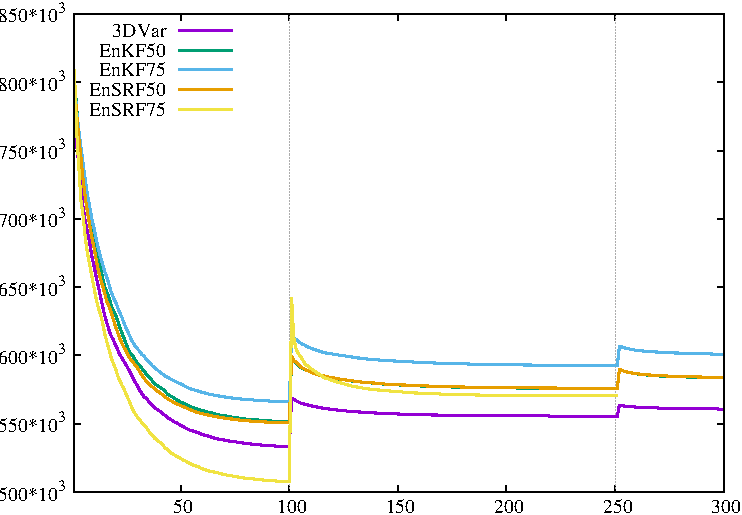
\includegraphics[width=0.47\textwidth]{./figs/cap4/fcost_exps_20130101_00-crop.pdf}
        }     
        \subfigure[06Z]{
            \label{fig:min_fcusto_06z}
            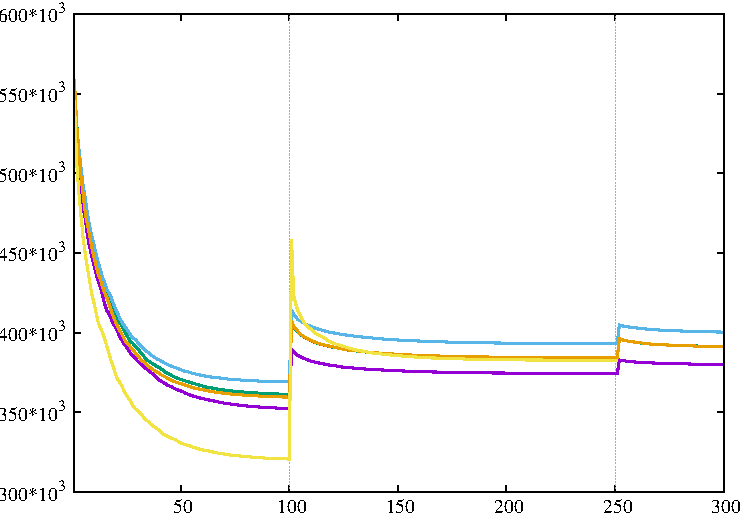
\includegraphics[width=0.47\textwidth]{./figs/cap4/fcost_exps_20130101_06-crop.pdf}
        }\\
        \subfigure[12Z]{
            \label{fig:min_fcusto_12z}
            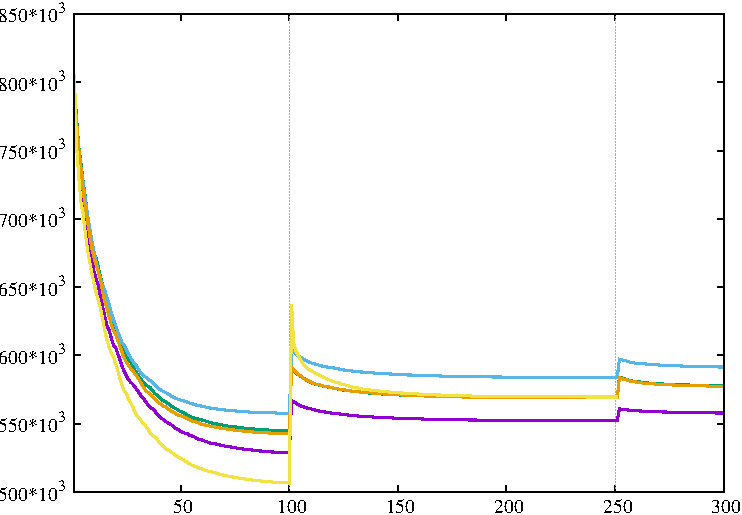
\includegraphics[width=0.47\textwidth]{./figs/cap4/fcost_exps_20130101_12-crop.pdf}
        }
        \subfigure[18Z]{
           \label{fig:min_fcusto_18z}
           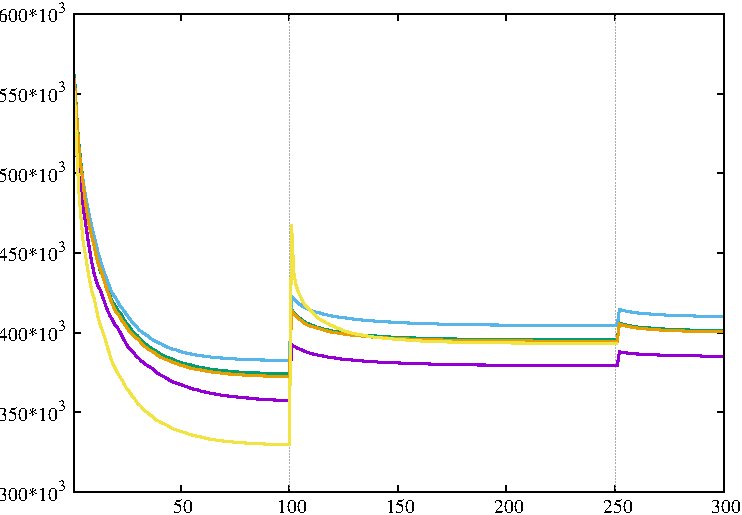
\includegraphics[width=0.47\textwidth]{./figs/cap4/fcost_exps_20130101_18-crop.pdf}
        }
    \end{center}
    \vspace{2mm}
    \legenda{Em \subref{fig:min_fcusto_00z} para as 00Z; \subref{fig:min_fcusto_06z} 06Z; \subref{fig:min_fcusto_12z} 12Z e \subref{fig:min_fcusto_18z} 18Z. No eixo $x$ estão representadas as iterações da minimização e estão destacados (linha pontilhada cinza) a parada das iterações internas e reinício das iterações externas.}
   \label{fig:min_fcusto_hsin}
   \FONTE{Produção do autor.}
\end{figure}

O método de minimização da função custo utilizado é o método do Gradiente Conjugado. Este método é o método padrão, mas há outras opções que podem ser testadas. O pré-condicionamento da função custo em aplicações operacionais é necessário para minimizar o custo computacional do cálculo da análise. Um opção é realizar o pré-condicionamento da minimização da função custo com base na matriz de covariâncias estática completa, ou com base na sua raiz quadrada. Em todos os experimentos realizados, foi utilizado, portanto, o método de minimização do gradiente conjugado com pré-condicionamento em $\mathbf{B}$ completa. No Apêndice \ref{apendiceII} é apresentada uma visão geral sobre o pré-condicionamento com base em $\mathbf{B}$ completa. 

\subsubsection*{Variável de Controle da Umidade}

A variável de controle de umidade no GSI pode ser escolhida de duas formas distintas: utilizando-se a pseudo-umidade relativa ou a umidade relativa normalizada. A escolha da variável de controle da umidade foi a umidade relativa normalizada porque esta representação permite que a umidade varie durante as iterações internas de acordo com as variações na pressão em superfície, temperatura e umidade específica. % incluir como referência o trabalho de Dee e da Silva.

\subsubsection*{Injunção de Umidade}

A implementação prática da função custo variacional, pode incluir outros termos além daqueles mostrados, e.g., na Eq. \ref{eq:32}. Um termo importante é o termo de injunção de umidade. Este termo é responsável por contabilizar e controlar a umidade negativa e supersaturada, que surgem devido aos modos computacionais e físicos envolvidos no processo de modelagem (i.e., prognóstico) e de análise. No GSI, dois parâmetros podem ser ajustados a fim de que a umidade não física possa ser controlada. O primeiro teste com a matriz de covariâncias na resolução TQ0062L028, mostrou-se instável (após poucos ciclos de análise). Vários testes foram realizados e, com base no trabalho de \citeonline{rodrigues/2017}, foi possível ajustar os seguintes valores: 5.0 para a umidade supersaturada e 0,005 para a umidade negativa. Nos testes realizados, notou-se que a magnitude destes valores podem ser relacionadas também com a resolução da grade da análise e modelo (neste caso, \textasciitilde{}200 km).

\subsection{Assimilação de Dados por Conjuntos}

Esta seção é dedicada a apresentar os principais parâmetros e aspectos relacionados com a aplicação do filtro de Kalman por conjunto, nas duas versões testadas (EnKF e EnSRF). Para ambos os algoritmos testados, as opções de localização do conjunto de previsões bem como a inflação (i.e., o \textit{inflation}) das covariâncias são as mesmas. Esta medida foi tomada para facilitar a comparação dos resultados obtidos. Entretanto, isso não significa que os sistemas devem ser realizados com as mesmas opções ou que não há necessidade de se ajustar adequadamente estas.

\subsubsection*{Determinação do Conjunto de Previsões Inicial}

Para a realização cíclica do sistema híbrido 3DVar utilizando os algorítmos EnKF ou EnSRF, um conjunto de previsões inicial é necessário, a partir do qual o filtro de Kalman por conjunto irá realizar a atualização das covariâncias a serem utilizadas em combinação com as covariâncias estáticas na minimização das função custo variacional. A metodologia empregada aqui é aquela semelhante ao \textit{poor man's ensemble} (e.g., \citeonline{ebert/2001,arribas/2005}), em que previsões independentes previamente realizadas por centros operacionais são utilizadas para se compor um conjunto de previsões para aplicações em previsões de curto a médio prazo. Entretanto, uma ideia semelhante foi aplicada aqui para se gerar um conjunto de previsões inicial para uso com o sistema híbrido 3DVar, o qual foi atualizado e propagado no tempo utilizando o filtro de Kalman por conjunto.

As etapas necessárias para se gerar um conjunto de previsões iniciais são as seguintes:

\begin{enumerate}
    \item Parte-se de uma análise determinística de resolução maior ou igual a resolução de interesse (i.e., pode-se partir de uma análise na resolução TQ0299L064 e realizar as previsões para a resolução TQ0062L028), realizam-se previsões a cada 12 horas para um período de 30 dias;
    \item Do conjunto de 60 previsões (2 previsões por dia), seleciona-se um subconjunto de previsões que representará o tamanho do conjunto;
    \item Renomeia-se os arquivos de forma que todos sejam válidos para o mesmo horário de previsão;
    \item Altera-se a data interna dos arquivos de forma que todos sejam efetivamente válidos para o horário de previsão desejado.
\end{enumerate}

Nas etapas acima, é necessário alterar-se a data interna dos arquivos de previsão, o que requer um programa que seja capaz de ler o arquivo de entrada, alterar a informação da data e horário da previsão no cabeçalho do arquivo e salvar estas informações junto com os coeficientes espectrais representados.

Para os experimentos realizados neste trabalho (Seção \ref{sec:exps}), foi utilizado um conjunto de 40 previsões iniciais, os quais se mostraram suficientes para a realização dos experimentos.

\subsubsection*{Localização do Conjunto de Análises}

A aplicação do filtro de Kalman por conjunto utilizando-se um conjunto de previsões relativamente pequeno para realizar a propagação dos estados e das suas covariâncias, pode fazer com que o filtro seja ineficiente e colapse. Isso pode ocorrer porque, à medida em que as observações são assimiladas no conjunto, o seu espalhamento tende a diminuir devido as inovações (e correções trazidas pelas observações). Isso implica em uma estimativa pobre das covariâncias dos erros de análise devido a um conjunto pequeno. Um conjunto pequeno contém alguns pouco membros (na ordem de 10 membros). Os 40 membros utilizados nos experimentos deste trabalho representam um número relativamente pequeno, mas suficiente para a realização dos experimentos propostos na resolução escolhida, sem se comprometer severamente a disponibilidade de tempo computacional e espaço para armazenamento.

A localização do conjunto de previsões é então utilizada para se compensar os efeitos da atualização cíclica de um conjunto que possui um espalhamento relativamente pequeno, devido ao seu tamanho. A implementação do EnKF no GSI, permite que sejam ajustados os seguintes parâmetros para se realizar a localização do conjunto de previsões:

\begin{itemize}
    \item Escala de localização horizontal do conjunto: 800 km;
    \item Escala de localização vertical do conjunto: 0,5 (unidades de grade).
\end{itemize}

Outra opção disponível para a localização do conjunto de previsões, é dada em função da razão entre a variância da análise no espaço das observações e a variância das previsões. Esta opção representa um valor limite para que as observações reduzam a variância do conjunto de previsões (e consequentemente manter parte do espalhamento do conjunto). O valor utilizado nesta opção foi de 98\%.

\subsubsection*{Inflação das Covariâncias}

Com a aplicação de um conjunto relativamente pequeno para a aplicação do filtro de Kalman por conjunto, as covariâncias derivadas do conjunto serão deficientes em posto (i.e., \textit{rank defficient}). Isso significa que, sendo a matriz de covariâncias do conjunto dimensionada no espaço do conjunto (i.e., uma de suas dimensões é a dimensão do conjunto, o seu tamanho), então não haverão elementos suficientes para uma adequada amostragem das variâncias e covariâncias dos erros das variáveis de estado. A inflação pode então ser utilizada (em diferentes regiões) com o objetivo de se inflar artificialmente estas covariâncias.

Na implementação do EnKF dentro do GSI, estão disponíveis as seguintes opções para a realização da inflação das covariâncias, as quais foram mantidas nos experimentos:

\begin{itemize}
    \item Parâmetro de inflação das covariâncias sobre o Hemisfério Norte: 85\%;
    \item Parâmetro de inflação das covariâncias sobre os Trópicos: 85\%;
    \item Parâmetro de inflação das covariâncias sobre o Hemisfério Sul: 85\%;
    \item Limite máximo de inflação (total): 100\%;
    \item Limite mínimo de inflação (total): 1\%.
\end{itemize}

\section{Ciclo de Assimilação de Dados do Sistema Híbrido Ensemble-Variacional}

O ciclo do sistema de assimilação de dados GSI é realizado alternando-se análises e previsões. Em modo de pesquisa, antes de se iniciar o ciclo, são gerados o primeiro conjunto de previsões e \textit{restarts} (que incluem a convecção, radiação e nuvens, dinâmica, - tempo corrente e passado - e superfície) do modelo de circulação geral do CPTEC, a partir dos quais, o ciclo é iniciado. Para isto, antes são preparados os campos fixos e a primeira condição inicial do modelo utilizando-se o pré-processamento. No ciclo, a primeira etapa, consiste do processamento das observações em um procedimento em que os arquivos de observações convencionais e não convencionais no formato PrepBUFR são preparados para leitura pelo GSI. Em seguida é executada a interface que converte a previsão de 9 horas do modelo do formato espectral para ponto de grade, preparando também para a leitura pelo GSI. Com as observações e previsões preparados, o GSI é executado e então a análise é determinada. Com a análise pronta, o modelo de circulação geral é então executado, lendo o \textit{restarts} gerado antes do ciclo, atualizando-se a Temperatura da Superfície do Mar (TSM) e a máscara de neve, prognosticando a dinâmica e diagnosticando a física do modelo conforme as configurações da Tabela \ref{tab:model}. Depois que o modelo escreve o resultado das previsões e escreve os \textit{restarts} para o próximo ciclo, o ciclo é reiniciado para o horário seguinte, realizando as mesmas etapas.

No diagrama da Figura \ref{fig:ciclohyb} é mostrado o ciclo de análises e previsões do sistema híbrido ensemble-variacional proposto. As equações em cada passo do ciclo são aquelas utilizadas pelo sistema de assimilação de dados híbrido para a determinação da análise. Neste diagrama, não estão representados o pré-processamento, interfaces, conversão das observações, mas apenas as partes principais. Para o ciclo de assimilação de dados híbrido, destacam-se as Eqs. \ref{eq:enkf_pb}, \ref{eq:29}, \ref{eq:30} e a função custo da Eq. \ref{eq:34}.

\begin{figure}[H]
  \vspace{-8mm}
  \caption{Diagrama esquemático do sistema híbrido 3DVar.}
  \vspace{2mm}
  \begin{center}
    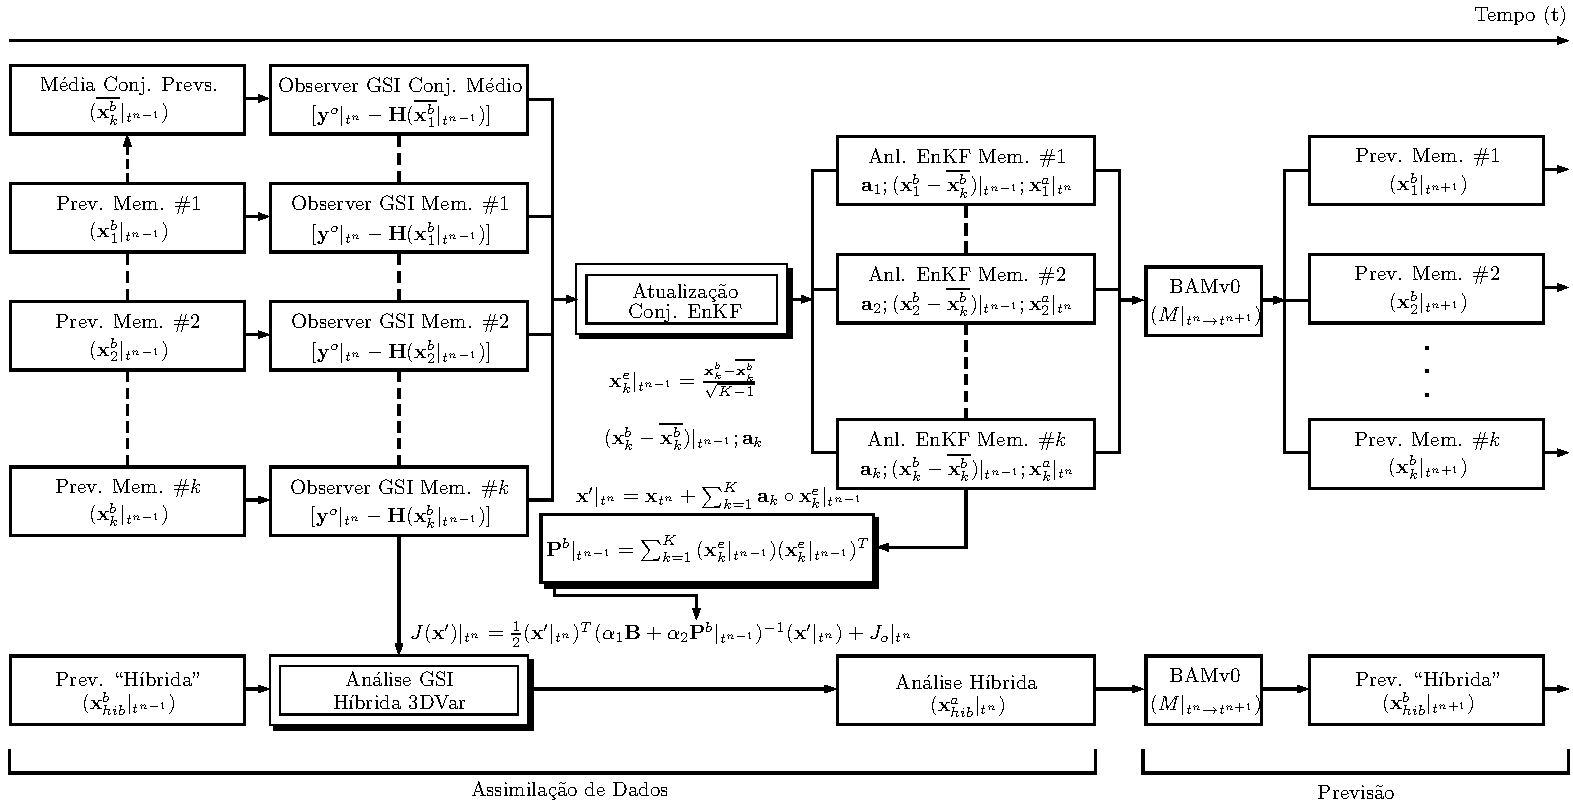
\includegraphics[scale=0.82,angle=90]{./figs/cap4/diagrama_hibrido_novo_pt-tempos.pdf}
  \end{center}
  \vspace{2mm}
  \legenda{As janelas de assimilação e previsão estão indicadas junto com o tempo de ocorrência das previsões, observações e análise (i.e., $t^{n-1}$, $t^{n}$, $t^{n+1}$). As equações referentes as etapas principais estão indicadas em suas respectivas posições.}
  \label{fig:ciclohyb}
  \FONTE{Produção do autor.}
\end{figure}

A Figura \ref{fig:ciclohyb} apresenta o ciclo de geração da análise híbrida 3DVar e a geração de um conjunto de $K$ membros. A análise híbrida é atualizada com a estimativa de covariância do erro de previsão estimada pela combinação entre a covariância estática do erro de previsão e a covariância do conjunto de $K$ membros. A perturbação do conjunto é então atualizada com inovações baseadas na inflação do conjunto aplicado. %\info{verificar}.

No sistema GSI, utilizando-se ou não a matriz de covariâncias estacionária, é dado o exemplo de como é calculada a análise do campo horizontal do vento. Este é um exemplo interessante, porque mostra o tratamento feito dentro do sistema em relação a variável de controle (divergência e vorticidade), a variável observada (componentes zonais do vento horizontal) e as quantidades tratadas dentro da matriz de covariâncias, importantes para a análise do vento (função de corrente e velocidade potencial).

\section{Exemplo da Análise do Campo de Vento Horizontal}
\label{sec:ex_anl_wind}

O modelo de circulação geral do CPTEC (seja o MCGAv4 ou o BAMv0, descritos na Seção \ref{sec:mcga}) prognostica a divergência ($D$) e a vorticidade ($\zeta$) para representar as componentes divergente e não divergente, respectivamente, do fluxo atmosférico. Na matriz de covariância, estão representas as covariâncias relacionadas ao vento em termos da função de corrente ($\psi$) e velocidade potencial ($\chi$). Em relação as observações de vento, diversos instrumentos são utilizados para a coleta de informações, mas são utilizadas pelo sistema de assimilação de dados (e também na matriz de covariância dos erros de observação) as componentes do vento horizontal, sendo representadas por meio das componentes zonal ($u$) e meridional ($v$) do vento.

Tomando-se por base a Eq.\ref{eq:fcusto} (desconsiderando os termos de injunção), temos:

\begin{equation}
    J(\mathbf{x}) = \frac{1}{2} (\mathbf{x} - \mathbf{x}^{b})^{T} \mathbf{B}^{-1} (\mathbf{x} - \mathbf{x}^{b}) + \frac{1}{2} [\mathbf{y}^{o}-\textit{H}(\mathbf{x}^{b})]^{T} \mathbf{R}^{-1} [\mathbf{y}^{o}-\textit{H}(\mathbf{x}^{b})]
\end{equation}

O problema de análise, seguindo a função custo da Eq. \ref{eq:fcusto}, pode ser dividido em duas partes: a primeira, relacionada ao termo de inovação da função custo (i.e., o termo $\mathbf{y}^{o}-\textit{H}(\mathbf{x}_{b})$), e a segunda parte, relacionada ao termo referente ao incremento de análise (i.e., o termo $\mathbf{x} - \mathbf{x}^{b}$).

Considerando que o incremento de análise é obtido quando o gradiente de $J$ é igual a zero, ie., $\nabla_{\mathbf{x}}{J}=0$ quando $\mathbf{x}=\mathbf{x}^{a}$, temos que:

\begin{equation}
    0 =  (\mathbf{B}^{-1} + \mathbf{H}^{T}\mathbf{R}^{-1}\mathbf{H})(\mathbf{x}^{a}-\mathbf{x}^{b}) - (\mathbf{H}^{T}\mathbf{R}^{-1})[\mathbf{y}^{o}-\textit{H}(\mathbf{x}^{b})]
    \label{eq:gradzero}
\end{equation}

A Eq. \ref{eq:gradzero} acarreta na Equação do Incremento de Análise (vide Apêndice \ref{apendiceI}):

\begin{equation}
    \mathbf{x}^{a}-\mathbf{x}^{b} = (\mathbf{B}^{-1} + \mathbf{H}^{T}\mathbf{R}^{-1}\mathbf{H})^{-1} \{\mathbf{H}^{T}\mathbf{R}^{-1} [\mathbf{y}^{o}-\textit{H}(\mathbf{x}^{b})]\}
    \label{eq:incranl}
\end{equation}

Dentro do GSI, esta equação não é explicitamente resolvida, mas os termos são todos calculados. As etapas relacionadas ao cálculo do incremento de análise, são as seguinte:

%\info{por que? a função custo é resolvida, mas por que esta equação não é resolvida?}

\begin{enumerate}
    \item Utilizando as Eqs. \ref{eq:25} e \ref{eq:26}, $\mathbf{H}$ transforma $D$ e $\zeta$ do modelo para $u$ e $v$, e interpola para o ponto de observação;
    \item Com $u$ e $v$ do modelo interpolados para o ponto da observação, é calculada a inovação $\mathbf{y}^{o}-\textit{H}(\mathbf{x}_{b})$;
    \item A inovação é então dividida pelo erro da observação, $\mathbf{R}^{-1}[{\mathbf{y}^{o}-\textit{H}(\mathbf{x}^{b})}]$;
    \item Esta inovação normalizada pelo erro da observação, é então transformada novamente para $D$ e $\zeta$ (ie., as inovações das componentes $u$ e $v$ são transformadas novamente para $D$ e $\zeta$)  por $\mathbf{H}^{T}$, $\mathbf{H}^{T}{\mathbf{R}^{-1}}[{\mathbf{y}^{o}-\textit{H}(\mathbf{x}^{b})}]$. Este termo está representado no segundo coeficiente do lado direito da Eq. \ref{eq:gradzero}.
\end{enumerate}

Esta é a primeira parte do cálculo da análise do vento horizontal, referente ao termo de inovação. A segunda parte, é referente ao termo de incremento de análise e, além de envolver a matriz de covariâncias dos erros de observação ($\mathbf{R}$, que neste caso representa os erros das observações de $u$ e $v$), envolve também a matriz de covariâncias dos erros de previsão ($\mathbf{B}$, representando portanto, os erros associados as quantidades de $\psi$ e $\chi$). O coeficiente $(\mathbf{B}^{-1} + \mathbf{H}^{T}\mathbf{R}^{-1}\mathbf{H})^{-1}$, lado direito da Eq. \ref{eq:gradzero}), indica a matriz inversa da soma das matrizes $\mathbf{B}$ e $\mathbf{R}$, no espaço do modelo (ponto de grade). A matriz $\mathbf{B}$ utiliza a Função de Corrente ($\psi$) e a Velocidade Potencial ($\chi$). As Eqs. \ref{eq:27} e \ref{eq:28}, são então utilizadas para calcular $\psi$ e $\chi$ a partir de $D$ e $\zeta$, respectivamente, e então $\mathbf{B}$ é aplicada para o cálculo final do incremento de análise de $T$, $ps$ e $\chi$ em termos de $\psi$. Finalmente, os incrementos de $\psi$ e $\chi$ são transformados de volta em incrementos de $D$ e $\zeta$.

A equação a seguir organiza as informações apresentadas de acordo com a natureza das quantidades avaliada para a análise do vento horizontal.

\begin{equation*}
    \overwritered{\mathbf{x}^{a}-\mathbf{x}^{b}}{$D$, $\zeta$}
    = ( 
    \overwriteblue{\mathbf{B}^{-1}}{$\psi$, $\chi$}
    + 
    \mathbf{H}^{T} 
    \overwritegreen{\mathbf{R}^{-1}}{$u$, $v$}
    \mathbf{H} )^{-1} \{ \mathbf{H}^{T} 
    \overwritegreen{\mathbf{R}^{-1}}{$u$, $v$}
    [ 
    \overwritegreen{\mathbf{y}^{o}}{$u$, $v$}
    - \textit{H} ( 
    \overwritered{\mathbf{x}^{b}}{$D$, $\zeta$}
    ) ] \}
\end{equation*} 

%\subsection{Custo Computacional}
%
%Neste trabalho de tese de doutorado, serão utilizados dois sistemas de assimilação de dados: o GSI (operacional no CPTEC) e o LETKF (pesquisa no CPTEC), além do MCGA-CPTEC/INPE. A aplicação destes modelos possui um custo computacional e esta seção tem por objetivo apresentar uma prospecção deste custo. Atualmente, o CPTEC conta com um supercomputador Cray XE6 com 1304 nós computacionais (cada nó possui 2 processadores AMD Opteron de 2,6 GHz de 6 núcleos cada) e 32 GB de memória compartilhada por nó e uma capacidade total de 258 teraflops de processamento. Este trabalho deverá ser desenvolvido dentro das quotas de utilização do supercomputador que o Grupo de Desenvolvimento em Assimilação de Dados do CPTEC possui, que é de $\sim$125TB de armazenamento distribuídos entre os discos online6, stornext/grupos e scratchin.
%
%As análises operacionais do GSI com o sistema de observação operacional, leva aproximadamente 15 minutos para ficar pronto e ocupa aproximadamente 150MB de espaço em disco por ciclo. O background do GSI (9 horas de previsão, TQ0299L028) leva aproximadamente 20 minutos para ficar pronto e ocupa aproximadamente 6GB de espaço em disco (contabilizando restarts e previsões). Uma análise do LETKF na resolução TQ0062L028 com 40 membros (mais o membro médio) leva aproximadamente 5 minutos para ficar pronto e ocupa cerca de 420MB de espaço em disco, por ciclo. Portanto, 1 ciclo do sistema híbrido LETKF-GSI pode levar aproximadamente 40 minutos (sem contar com otimizações e adequações de scripts e rotinas), considerando-se todos os processos envolvidos e na resolução TQ0299L064 (sendo esta a melhor resolução da análise variacional híbrida final). O armazenamento, inclui as análises, previsões e arquivos pré  e pós-processados, além dos arquivos de observação e de interface (arquivos convertidos entre as soluções espectral e em ponto de grade e vice-versa). Tudo isso soma cerca de 10GB por ciclo. Extrapolando-se para 5 experimentos de 120 ciclos cada um (1 mês, 4 ciclos por dia), no total, serão necessários cerca de 2TB de espaço em disco e 8 horas de processamento por experimento.

\section{Experimentos com o Sistema Híbrido 3DVar}
\label{sec:exps}

Uma das principais características do sistema híbrido 3DVar, é a capacidade de combinar covariâncias estáticas e covariâncias provenientes de um conjunto de previsões. Tal como foi apresentado nas seções anteriores, os coeficientes $\alpha_{1}$ e $\alpha_{2}$ podem ser utilizados para se ponderar a quantidade de contribuição destas covariâncias que serão utilizadas na minimização da função custo variacional. Com o objetivo de se exercitar e avaliar o sistema híbrido 3DVar em ciclos de assimilação de dados utilizando os dados de observações sumarizados na Tabela \ref{tab:mobs}, foram elaborados dois grupos de experimento. O primeiro grupo é composto por dois experimentos que serão utilizados como controle; o segundo grupo é composto por 4 experimentos que representam o sistema híbrido 3DVar. 

Na Tabela \ref{tab:exps} são apresentados os experimentos dos grupos 1 e 2, e apresenta as características principais de cada um deles.

\begin{table}[H]
\caption{Experimentos com o sistema híbrido 3DVar.}
\begin{center} 
\begin{tabular}{cccc}
\toprule
\toprule
\multicolumn{1}{c}{\textbf{Experimento}} & \multicolumn{1}{c}{\textbf{Ajuste das Covariâncias}} & \multicolumn{1}{c}{\textbf{Descrição}} \\
\midrule
\multicolumn{1}{c}{REF}     & \multicolumn{1}{c}{--}                 & -- \\
\multicolumn{1}{c}{3DVar}   & \multicolumn{1}{c}{--}                 & \multicolumn{1}{c}{$\mathbf{B}$ (BAMv0, 730 pares)} \\ 
\multicolumn{1}{c}{EnKF50}  & \multicolumn{1}{p{5cm}}{50\% Estático ($\alpha_{1}=0,5$)} & \multicolumn{1}{c}{$\mathbf{B}$ (BAMv0, 40 membros)} \\ 
\multicolumn{1}{c}{EnKF75}  & \multicolumn{1}{p{5cm}}{75\% Conjunto ($\alpha_{1}=0,25$)} & \multicolumn{1}{c}{$\mathbf{B}$ (BAMv0, 40 membros)} \\ 
\multicolumn{1}{c}{EnSRF50} & \multicolumn{1}{p{5cm}}{50\% Estático ($\alpha_{1}=0,5$)} & \multicolumn{1}{c}{$\mathbf{B}$ (BAMv0, 40 membros)} \\ 
\multicolumn{1}{c}{EnSRF75} & \multicolumn{1}{p{5cm}}{75\% Conjunto ($\alpha_{1}=0,25$)} & \multicolumn{1}{c}{$\mathbf{B}$ (BAMv0, 40 membros)} \\ 
\bottomrule
\end{tabular}
\end{center}
\label{tab:exps}
\end{table}

O objetivo do experimento REF é servir como referência para todos os experimentos que envolvem ciclos de assimilação de dados, de forma que se possa conhecer as diferenças entre realizar o modelo de circulação geral do CPTEC com e sem os ciclos de assimilação de dados. Para que seja, portanto, possível se comparar o desempenho dos experimentos híbridos, realizou-se também um experimento cíclico com o sistema 3DVar puro, de forma que este sirva como base para as comparações com as contribuições das covariâncias dos conjuntos de previsões. Os experimentos EnKF50 (EnKF75) e EnSRF50 (EnSRF75), são os experimentos que utilizarão o conjunto de 40 membros de previsões com o EnKF e EnSRF, com 50\% e 75\% de contribuição das covariâncias do conjunto, as covariâncias estáticas.